
	\documentclass[16pt,a4paper,oneside]{article}
	\usepackage[utf8]{inputenc}
	\usepackage{amsmath}
	\usepackage{amsfonts}
	\usepackage{amssymb}
	\usepackage{amsmath}
	\usepackage{a4wide}
	\usepackage{array}
	\usepackage{epsfig}
	\usepackage{amsfonts}
	\usepackage{cite}
	\usepackage{amssymb}
	\usepackage{scrextend}
	\changefontsizes{12pt}

	\usepackage{tikz}
\usepackage[a4paper,left=1.5cm,right=1.5cm,top=2.0cm,bottom=2.0cm]{geometry}
	\usetikzlibrary{matrix,calc}
	\usepackage{setspace}
	\usepackage{tikz-timing}[2009/12/09]
	\def\degr{${}^\circ$}
	\usepackage{epsfig}
	\usepackage{multirow}
	\usetikzlibrary{calc}
	\usepackage{multicol}
	\usepackage{xcolor}
	\usepackage{vietnam}
	\usepackage{float} 
	\usepackage{cases} 
	\usepackage{graphicx}
	\usepackage{indentfirst}
	\usepackage{fancyhdr}
	\pagestyle{fancy}
	\usepackage{utopia}
	\lhead{
\includegraphics[width=0.5cm]{hcmut.png}}
	\chead{}

	\lhead{\textbf{KỸ THUẬT LẬP TRÌNH}}
	\cfoot{\thepage}
	\rhead{\textbf{BÀI TẬP LỚN 02}}
	\renewcommand{\headrulewidth}{0.4pt}
	\renewcommand{\footrulewidth}{0.4pt}
	\fontsize{80pt}{80pt}\selectfont
	%%%%%%%%%%%%%%%%%%%%%%%%%%%%%%%%%%%%%%%%%% Phần định nghĩa mấy cái để vẽ Kmap
	
	%Nhóm 1 vùng nối liền
	\newcommand{\noilien}[4][0]{
		\draw[rounded corners=3pt, fill=#4, opacity=.3] ($(#2.north west)+(135:#1)$) rectangle ($(#3.south east)+(-45:#1)$);
	}
	%Nhóm trái-phải
	\newcommand{\traiphai}[4][0]{
		\draw[rounded corners=3pt, fill=#4, opacity=.3] ($(rf.east |- #2.north)+(90:#1)$)-| ($(#2.east)+(0:#1)$) |- ($(rf.east |- #3.south)+(-90:#1)$);
		\draw[rounded corners=3pt, fill=#4, opacity=.3] ($(cf.west |- #2.north)+(90:#1)$) -| ($(#3.west)+(180:#1)$) |- ($(cf.west |- #3.south)+(-90:#1)$);
	}
	
	%Nhóm trên-dưới
	\newcommand{\trenduoi}[4][0]{
		\draw[rounded corners=3pt, fill=#4, opacity=.3] ($(cf.south -| #2.west)+(180:#1)$) |- ($(#2.south)+(-90:#1)$) -| ($(cf.south -| #3.east)+(0:#1)$);
		\draw[rounded corners=3pt, fill=#4, opacity=.3] ($(rf.north -| #2.west)+(180:#1)$) |- ($(#3.north)+(90:#1)$) -| ($(rf.north -| #3.east)+(0:#1)$);
	}
	%Nhóm bốn góc
	\newcommand{\bongoc}[2][0]{
		\draw[rounded corners=3pt, fill=#2, opacity=.3] ($(rf.east |- 0.south)+(-90:#1)$) -| ($(0.east |- cf.south)+(0:#1)$);
		\draw[rounded corners=3pt, fill=#2, opacity=.3] ($(rf.east |- 8.north)+(90:#1)$) -| ($(8.east |- rf.north)+(0:#1)$);
		\draw[rounded corners=3pt, fill=#2, opacity=.3] ($(cf.west |- 2.south)+(-90:#1)$) -| ($(2.west |- cf.south)+(180:#1)$);
		\draw[rounded corners=3pt, fill=#2, opacity=.3] ($(cf.west |- 10.north)+(90:#1)$) -| ($(10.west |- rf.north)+(180:#1)$);
	}
	
	
	%Định nghĩa Knaughmap 4x4
	\newenvironment{Karnaugh}[2]%
	{
		\begin{tikzpicture}[baseline=(current bounding box.north),scale=0.8]
		\draw (0,0) grid (4,4);
		\draw (0,4) -- node [pos=0.7,above right,anchor=south west] {#2} node [pos=0.7,below left,anchor=north east] {#1} ++(135:1);
		%
		\matrix (mapa) [matrix of nodes,
		column sep={0.8cm,between origins},
		row sep={0.8cm,between origins},
		every node/.style={minimum size=0.3mm},
		anchor=8.center,
		ampersand replacement=\&] at (0.5,0.5)
		{
			\& |(c00)| 00         \& |(c01)| 01         \& |(c11)| 11         \& |(c10)| 10         \& |(cf)| \phantom{00} \\
			|(r00)| 00             \& |(0)|  \phantom{0} \& |(1)|  \phantom{0} \& |(3)|  \phantom{0} \& |(2)|  \phantom{0} \&                     \\
			|(r01)| 01             \& |(4)|  \phantom{0} \& |(5)|  \phantom{0} \& |(7)|  \phantom{0} \& |(6)|  \phantom{0} \&                     \\
			|(r11)| 11             \& |(12)| \phantom{0} \& |(13)| \phantom{0} \& |(15)| \phantom{0} \& |(14)| \phantom{0} \&                     \\
			|(r10)| 10             \& |(8)|  \phantom{0} \& |(9)|  \phantom{0} \& |(11)| \phantom{0} \& |(10)| \phantom{0} \&                     \\
			|(rf) | \phantom{00}   \&                    \&                    \&                    \&                    \&                     \\
		};
	}
	{
		\end{tikzpicture}
	}
	%%%%%%%%%%%
	\newcommand{\contingut}[1]{%
		\foreach \x [count=\xi from 0]  in {#1}
		\path (\xi) node {\x};
	}
	\newcommand{\implicantsol}[3][0]{
		\draw[rounded corners=3pt, fill=#3, opacity=.3] ($(#2.north west)+(135:#1)$) rectangle ($(#2.south east)+(-45:#1)$);
	}
	
	
	
	\newcommand{\implicant}[4][0]{
		\draw[rounded corners=3pt, fill=#4, opacity=.3] ($(#2.north west)+(135:#1)$) rectangle ($(#3.south east)+(-45:#1)$);
	}
	
	
	\newcommand{\implicantcostats}[4][0]{
		\draw[rounded corners=3pt, fill=#4, opacity=.3] ($(rf.east |- #2.north)+(90:#1)$)-| ($(#2.east)+(0:#1)$) |- ($(rf.east |- #3.south)+(-90:#1)$);
		\draw[rounded corners=3pt, fill=#4, opacity=.3] ($(cf.west |- #2.north)+(90:#1)$) -| ($(#3.west)+(180:#1)$) |- ($(cf.west |- #3.south)+(-90:#1)$);
	}
	
	\newcommand{\implicantdaltbaix}[4][0]{
		\draw[rounded corners=3pt, fill=#4, opacity=.3] ($(cf.south -| #2.west)+(180:#1)$) |- ($(#2.south)+(-90:#1)$) -| ($(cf.south -| #3.east)+(0:#1)$);
		\draw[rounded corners=3pt, fill=#4, opacity=.3] ($(rf.north -| #2.west)+(180:#1)$) |- ($(#3.north)+(90:#1)$) -| ($(rf.north -| #3.east)+(0:#1)$);
	}
	
	\newcommand{\implicantcantons}[2][0]{
		\draw[rounded corners=3pt, opacity=.3] ($(rf.east |- 0.south)+(-90:#1)$) -| ($(0.east |- cf.south)+(0:#1)$);
		\draw[rounded corners=3pt, opacity=.3] ($(rf.east |- 8.north)+(90:#1)$) -| ($(8.east |- rf.north)+(0:#1)$);
		\draw[rounded corners=3pt, opacity=.3] ($(cf.west |- 2.south)+(-90:#1)$) -| ($(2.west |- cf.south)+(180:#1)$);
		\draw[rounded corners=3pt, opacity=.3] ($(cf.west |- 10.north)+(90:#1)$) -| ($(10.west |- rf.north)+(180:#1)$);
		\fill[rounded corners=3pt, fill=#2, opacity=.3] ($(rf.east |- 0.south)+(-90:#1)$) -|  ($(0.east |- cf.south)+(0:#1)$) [sharp corners] ($(rf.east |- 0.south)+(-90:#1)$) |-  ($(0.east |- cf.south)+(0:#1)$) ;
		\fill[rounded corners=3pt, fill=#2, opacity=.3] ($(rf.east |- 8.north)+(90:#1)$) -| ($(8.east |- rf.north)+(0:#1)$) [sharp corners] ($(rf.east |- 8.north)+(90:#1)$) |- ($(8.east |- rf.north)+(0:#1)$) ;
		\fill[rounded corners=3pt, fill=#2, opacity=.3] ($(cf.west |- 2.south)+(-90:#1)$) -| ($(2.west |- cf.south)+(180:#1)$) [sharp corners]($(cf.west |- 2.south)+(-90:#1)$) |- ($(2.west |- cf.south)+(180:#1)$) ;
		\fill[rounded corners=3pt, fill=#2, opacity=.3] ($(cf.west |- 10.north)+(90:#1)$) -| ($(10.west |- rf.north)+(180:#1)$) [sharp corners] ($(cf.west |- 10.north)+(90:#1)$) |- ($(10.west |- rf.north)+(180:#1)$) ;
	}
	
	%Điền 8 or 16 giá trị vào các ô (0,1,X)
	\newcommand{\dienso}[1]{%
		\foreach \x [count=\xi from 0]  in {#1}
		\path (\xi) node {\x};
	}
	%%%%%%%%%%%%%%%%%%%%%%%%%%%%%%%%%%%%%%%%%%%%%%%%%%%%%%%%%%%%%%%%%%%%%%%%%%%%
	\newenvironment{Karnaughvuit}[2]%
	{
		\begin{tikzpicture}[baseline=(current bounding box.north),scale=0.8]
		\draw (0,0) grid (2,4);
		\draw (0,4) -- node [pos=0.7,above right,anchor=south west] {#2} node [pos=0.7,below left,anchor=north east] {#1} ++(135:1);
		%
		\matrix (mapa) [matrix of nodes,
		column sep={0.8cm,between origins},
		row sep={0.8cm,between origins},
		every node/.style={minimum size=0.3mm},
		anchor=4.center,
		ampersand replacement=\&] at (0.5,0.5)
		{
			\& |(c00)| 0         \& |(c01)| 1           \& |(cf)| \phantom{00} \\
			|(r00)| 00             \& |(0)|  \phantom{0} \& |(1)|  \phantom{0} \&                     \\
			|(r01)| 01             \& |(2)|  \phantom{0} \& |(3)|  \phantom{0} \&                     \\
			|(r11)| 11             \& |(6)|  \phantom{0} \& |(7)|  \phantom{0} \&                     \\
			|(r10)| 10             \& |(4)|  \phantom{0} \& |(5)|  \phantom{0} \&                     \\
			|(rf) | \phantom{00}   \&                    \&                    \&                     \\
		};
	}%
	{
		\end{tikzpicture}
	}
	%%%%%%%%%%%
	\begin{document}
		\begin{titlepage}
			\thispagestyle{empty}
			\begin{tikzpicture}[remember picture, overlay]%vẽ khung
			\draw[line width = 3pt] ($(current page.north west) + (0.65in,-0.5in)$) rectangle ($(current page.south east) + (-0.65in,0.5in)$);
			\end{tikzpicture}
			\begin{center}
				\large \textbf{\fontsize{12pt}{12pt}\selectfont ĐẠI HỌC BÁCH KHOA THÀNH PHỐ HỒ CHÍ MINH}\\
				\large \textbf{\fontsize{12pt}{12pt}\selectfont KHOA HỌC VÀ KỸ THUẬT}\\
				\large \textbf{\fontsize{12pt}{12pt}\selectfont MÁY TÍNH}\\
				\vspace{0.25cm}
				\begin{figure}[htp]
					\centering					
\includegraphics[width=4cm, height=4cm]{Images/hcmut.png}
				\end{figure}
			\end{center}
			\vspace{2cm}
			\begin{center}
				 \textcolor{blue}{	\Huge \textbf{\fontsize{29pt}{29pt}\selectfont  KỸ THUẬT LẬP TRÌNH}}\\
				\vspace{1cm}

				\huge \underline{\textbf{BÁO CÁO BÀI TẬP LỚN 02}}\\
				\vspace{1cm}

			\end{center}
			\vspace{1.5cm}
			\begin{center}
					\begin{table}[h]
					\begin{tabular}{rrl}
						\hspace{3 cm}	  & \text{ \color{blue} Giáo viên hướng dẫn:} & \textbf{ Lê Thành Sách}\\
						& & \textbf{Nguyễn Đức Dũng}\\
						&$~~~$&$~~$\\
												&$~~~$&$~~$\\
						& \text{ \color{blue} NHÓM L3T  GỒM:}	& Nguyễn Minh Thám $~~~~~~~~~~~~~$ $~~$1613166\\
						& &	Phạm Cao Lương $~~~~~~~~~~~~~~~~~~~~~$ 1611949\\
						& & Nguyễn Hữu Đức Thành $~~~~~~$  1613188\\
						& & Nguyễn Ngọc Đức Tâm $~~~~~~~~~$  1613055
					
						
					
					\end{tabular}
				\end{table}
				
			\end{center}
			\vspace{2cm}
			\begin{center}
				TP.Hồ Chí Minh, ngày 20, tháng 6, năm 2017
			\end{center}
		\end{titlepage}
		\newpage
\tableofcontents
\newpage
\section{Hướng dẫn sử dụng phần mềm}
\begin{itemize}
	\item Nếu bạn là một người mới sử dụng phần mềm của chúng tôi (chưa phải là người dùng ), thì bạn chỉ có thể sử dụng một số tính năng như ở MENU LIBPRO. 
	\item Bạn muốn sử dụng các tính năng khác của phần mềm thì cần phải đăng kí trở thành người dùng của phần mềm. Khi đó, bạn có thể sử dụng thêm các tính năng mới ở MENU USER.
	\item Khi bạn tạo một tài khoản và được xét duyệt thành công thì bạn có thể sử dụng các tính năng mà tài khoản đó được cấp. Cụ thể, tài  khoản bạn sẽ được cung cấp các vai trò sau:
	\begin{itemize}
		\item Độc giả
		\item Quản lý người dùng
		\item Thủ thư
		\item Độc giả và quản lý người dùng
		\item Độc giả và thủ thư
		\item Quản lý người dùng và thủ thư
		\item Độc giả, quản lý người dùng và thủ thư.
	\end{itemize}
\item Với mỗi vai trò khác nhau thì sẽ in ra các menu tương ứng. 
\item \underline{\textbf{Lưu ý: }} Khi bạn vừa vào phần mềm thì hệ thống sẽ tự động gửi thông báo nhắc nhở trả sách cho các độc giả khi còn đúng 5 ngày nữa là hết hạn trả sách.
\end{itemize}
\subsection{Menu LIBPRO}
\begin{figure}[htp]
	\begin{center}
		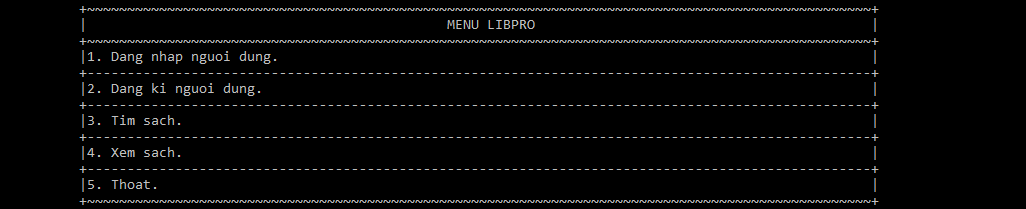
\includegraphics[width=18cm]{Images/menu_libpro.png}
		\caption{MENU LIBPRO}
	\end{center}
\end{figure}
	\renewcommand{\labelitemi}{$\blacksquare$}
\begin{itemize}
	\item \underline{\textit{Đăng nhập người dùng:}}\\
	Bạn sẽ đăng nhập người dùng bằng 2 thông tin là tên người dùng bạn đăng kí và số thứ tự người dụng hệ thống cung cấp cho bạn. Sau khi đăng nhập thành công thì bạn sẽ chuyển qua MENU dành cho người dùng để được sử dụng các tính năng của người dùng.
	\item \underline{\textit{Đăng kí người dùng.}}\\
	Bạn có thể đăng kí người dùng và có thể đăng nhập được ngay để sử dụng các tính năng cung cấp cho người dùng. Khi đăng kí người dùng bạn ghi các thông tin:
	\begin{itemize}
		\item \textit{Tên người dùng}.
		\item \textit{Số thự tự người dùng} (có 4 ký tự):$~~$ Ở đây bạn không cần điền vào mà hệ thống sẽ tự cung cấp số thự tự của bạn bằng cách lấy số thự tự của người dùng đăng kí sau cùng cộng 1.
		\item \textit{Mã số sinh viên}:$~~$ Đây là thông tin quan trọng để giúp hệ thống tránh việc một người có nhiều người dùng trong phần mềm. Cho nên mã số sinh viên bạn nhập vào phải khác với tất cả các mã số sinh viên đã đăng kí trong hệ thống.
		\item \textit{Ngày, tháng, năm sinh: }$~~$ Bạn sẽ nhập năm sinh của mình dưới dạng dd-mm-yyyy , ví dụ: 22-06-2017. Nếu không nhập đúng định dạng này hoặc nhập các ngày, tháng không có trong năm thì hệ thống sẽ yêu cầu bạn nhập lại.
		\item \textit{Nghề nghiệp.}
		\item \textit{Email: }$~~$ Thông tin này sẽ cũng giống như mã số sinh viên, nó sẽ giúp hệ thống tránh việc có nhiều người dùng của cùng 1 người. Bạn sẽ nhập email khác với email của tất cả các email đã đăng kí trước đó và email này chỉ được dưới dạng: @gmail.com, @gmail.com.vn, @hcmut.edu.vn, @yahoo.com.
	\end{itemize}
	\item \underline{\textit{Tìm sách}}\\
		Bạn được quyền xem tất cả sách có trong thư viện bao gồm các thông tin: ID sách, tên sách, tác giả, thể loại.
	\item \underline{\textit{Xem sách.}}\\
	Bạn có thể tìm sách theo tên sách mà tài khoản mong muốn. Hoặc khi bạn không nhớ hết tên sách mình muốn tìm kiếm thì cũng có thể tìm kiếm sách bằng cách nhập một số từ của tên sách mà bạn nhớ được.
	\item \underline{\textit{Thoát.}}\\
	Ở đây bạn có thể thoát ngay ra khỏi phần mềm mà không phải chuyển qua các menu nào khác. Lưu ý: Chỉ có duy nhất tính năng THOÁT ở menu này sẽ thoát khỏi phần mềm.
\end{itemize}
\subsection{Menu dành cho người dùng}
\begin{figure}[htp]
	\begin{center}
		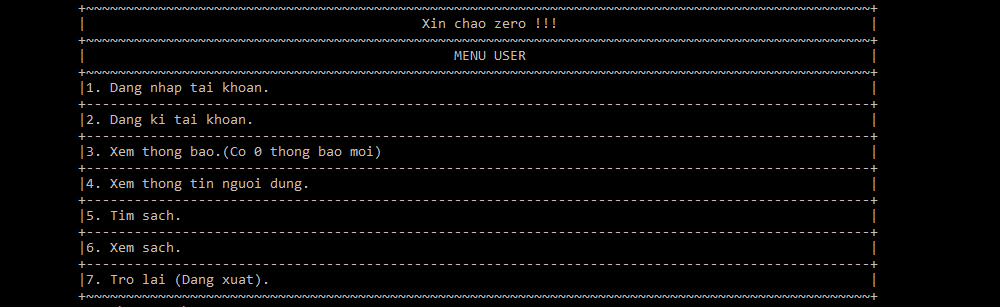
\includegraphics[width=18cm]{Images/menu_user.png}
		\caption{MENU USER}
	\end{center}
\end{figure}
\begin{itemize}
\item \underline{\textit{Đăng nhập tài khoản.}}\\
\begin{itemize}
\item Bạn đăng nhập tài khoản bằng cách nhập tên tài khoản và mật khẩu của tài khoản đó. Sau đó hệ  thống sẽ kiểm tra tài khoản của bạn có vai trò gì rồi sau đó sẽ in ra MENU của vài trò đó để bạn tương tác. (hệ thống sẽ kiểm tra xem tài khoản bạn có ở tình trạng hoạt động không)
\item Nếu bạn quên mật khẩu của tài khoản thì có thể chọn tính năng "Quên mật khẩu". Khi đó, hệ sẽ yêu cầu bạn điền các thông tin sau: ID người dùng bạn đang đăng nhập, mã số sinh viên, email của người dùng và cuối cùng tên tài khoản bạn muốn đổi mật khẩu. Yêu cầu này sẽ được gửi đến người QUẢN LÝ. Sau khi người người quan lý chấp nhận và reset mật khẩu cho tài khoản của bạn thì mật khẩu này sẽ được gửi đến phần THÔNG BÁO bến dưới. 
\end{itemize}
\item \underline{\textit{Đăng kí tài khoản}}\\
Hệ thống sẽ yêu cầu điền các thông tin:
\begin{itemize}
	\item \textit{Tên tài khoản: }Tài khoản này phải khác với tên tất cả tài khoản có trong hệ thống.
	\item \textit{Mật khẩu: }Bạn sẽ nhập mật khẩu của mình và được nhập lại một lần nữa để xác nhận.
	\item \textit{Chọn vai trò: }Hệ thống sẽ cho bạn chọn một trong 7 vai trò (Độc giả, thủ thư, quản lý người dùng và tổ hợp của 3 vai trò này) mà bạn mong muốn người quản lý khi xét duyệt yêu cầu đăng kí tài khoản sẽ cung cấp cho bạn.
\end{itemize}
\item \underline{\textit{Xem thông báo.}}\\
Hệ thống sẽ tự động cho bạn biết có bao nhiêu thông báo mới được gửi đến bạn. Khi bạn xem xong các thông báo mới này, thì các thông báo này sẽ được chuyển vào phần thông báo cũ (bạn cũng có thể xem các thông báo cũ này).\\
Các thông báo này có thể về:
\begin{itemize}
	\item Sách mới về: Khi người thu thư thêm sách vào thư viện thì hệ thống sẽ thông báo cho bạn.
	\item Khi tài khoản bạn được người quản lý chấp nhận và reset mật khẩu thì hệ thống sẽ thông báo cho bạn biết.
	\item Khi người quản lý thêm một tài khoản bất kỳ vào người dùng của bạn thì hệ thống sẽ thông báo tên tài khoản và mật khẩu của tài khoản đó.
\end{itemize}
\item \underline{\textit{Xem thông tin người dùng.}}\\
Hệ thống sẽ in ra các thông tin người dùng như: , ,  năm sinh,
\begin{itemize}
	\item ID người dùng.
	\item Tên người dùng.
	\item Mã số sinh viên người dùng.
	\item Ngày, tháng , năm sinh.
	\item Nghề nghiệp
	\item Email
	\item Danh sách cái tài khoản: tên tài khoản, vai trò, tình trạng của tài khoản(true hoặc false).
\end{itemize}
\item \underline{\textit{Trở lại}}\\
Hệ thống sẽ in ra MENU LIBPRO.
\end{itemize}
\subsection{Menu dành cho Độc giả}
\begin{figure}[htp]
	\begin{center}
		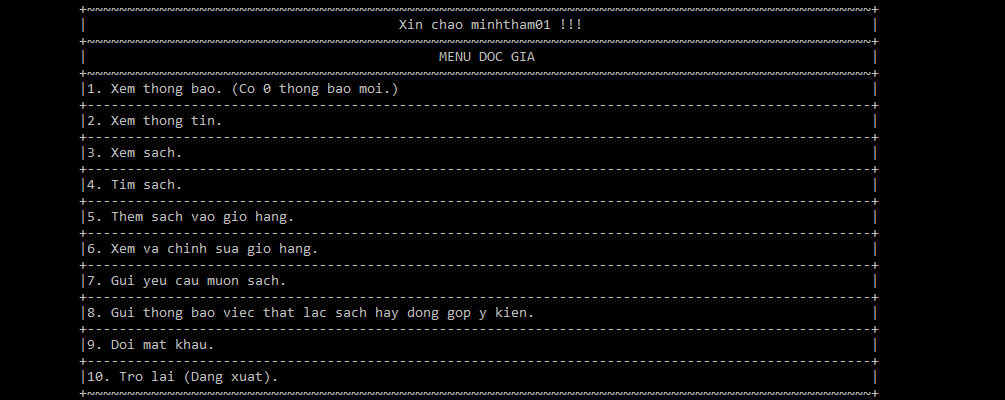
\includegraphics[width=18cm]{Images/menu_docgia.png}
		\caption{MENU ĐỘC GIẢ}
	\end{center}
\end{figure}
\begin{itemize}
	\item \underline{\textit{Xem thông báo:}}\\
	Hệ thống sẽ tự động cho bạn biết có bao nhiêu thông báo mới được gửi đến bạn. Khi bạn xem xong các thông báo mới này, thì các thông báo này sẽ được chuyển vào phần thông báo cũ (bạn cũng có thể xem các thông báo cũ này).\\
	 Các thông báo này có thể về:
	\begin{itemize}
		\item Sách mới về.
		\item Câu trả lời (hay hình thức phạt) của thủ thư khi bạn gửi  thông báo việc thất lạc sách hay đóng góp ý kiến để phát triển chương trình tốt hơn.
		\item Hệ thống sẽ tự động thông báo việc trả sách cho bạn (trước 5 ngày của hạn cuối cùng trả sách).
	\end{itemize}
	\item \underline{\textit{Xem thông tin:}}\\
	Tài khoản có thể xem được lịch sử của:
	\begin{itemize}
		\item Các lần gửi yêu cầu mượn sách.
		\item Các lần đã mượn sách: chưa trả, trả rồi, quá hạn mượn sách.
	\end{itemize}	
	\item \underline{\textit{Thêm sách vào giỏ hàng.}}\\
	Khi bạn vào tính năng này thì hệ thống sẽ in ra danh sách tất cả sách của thư viện. Bạn có thể chọn các sách mình muốn mượn vào giỏ hàng (chọn theo id sách) và số sách cần mượn. Số sách tối đa có thể thêm vào giỏ hàng là 10. Ở đây, nếu bạn đã mượn sách nhưng chưa trả sách cho thư viện hay bạn đã gửi yêu cầu mượn sách trước đó thì hệ thống sẽ không cho bạn thêm sách vào giỏ hàng.
	\item \underline{\textit{Chỉnh sửa giỏ hàng.}}\\
	Bạn có thể xem lại giỏ hàng của mình và có quyền chỉnh sửa số lượng sách hay xóa những sách bạn không muốn mượn nữa.
	\item \underline{\textit{Gửi yêu cầu mượn sách.}}\\
	Hệ thống sẽ mời bạn nhập vào ngày bạn muốn mượn sách (ngày này phải lớn hơn ngày hiện tại bạn gửi cầu). Sau đó, hệ thống sẽ tự động tính hạn trả sách của bạn (tối đa là 30 ngày). Ở đây bạn có thể xác nhận lại một lần nữa các thông tin sách mình muốn mượn (các sách trong giỏ hàng), ngày mượn sách, hạn cuối trả sách.
	\item \underline{\textit{Gửi thông báo việc thất lạc sách, hoặc đóng góp ý kiến về chương trình.}}\\
	Bạn có thể gửi thông báo về việc thất lạc sách của mình cho thủ thư, để thủ thư có hình thức xử lý. Hoặc, bạn có thể gửi các ý kiến đóng góp về cách hoạt động của thư viện như thế nào. Thủ thư sẽ có trả lời cho bạn một cách sớm nhất.
	\item \underline{\textit{Đổi mật khẩu.}}\\
	Ở đây, bạn có thể đổi mật khẩu của mình nhưng bắt buộc phải nhớ mật khẩu cũ trước đó của bạn.
	\item \underline{\textit{Đăng xuất.(Thoát)}}\\
	Khi bạn chọn tính năng này thì bạn sẽ về Menu của người dùng. Khi đó các sách bạn muốn mượn lưu trong giỏ hàng sẽ bị xóa đi.
\end{itemize}

\subsection{Menu dành cho Quản lý người dùng}
\begin{figure}[htp]
	\begin{center}
		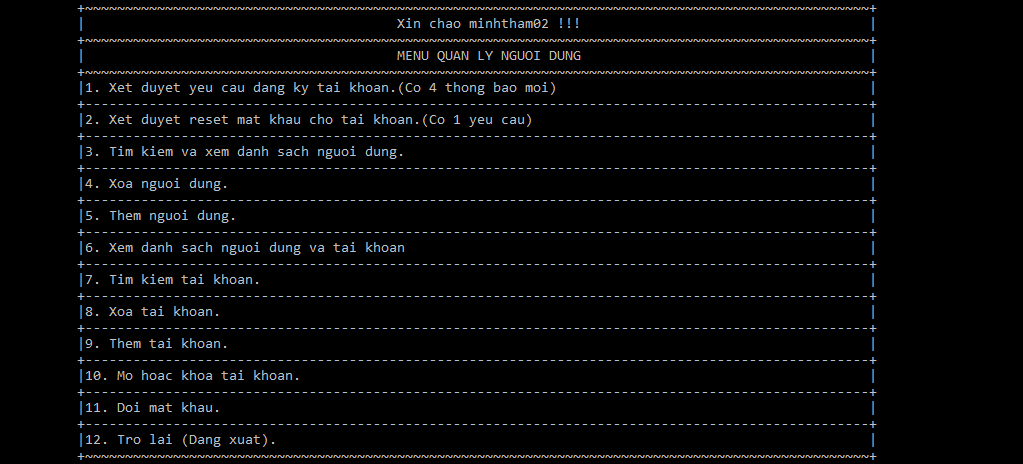
\includegraphics[width=18cm]{Images/menu_quanly.png}
		\caption{MENU QUẢN LÝ NGƯỜI DÙNG}
	\end{center}
\end{figure}
\begin{itemize}
	\item \underline{\textit{Xét duyệt yêu cầu đăng kí tài khoản.}}\\
		Hệ thống sẽ tự động cho bạn biết có bao nhiêu yêu cầu đăng kí tài khoản. Khi bạn chọn tính năng này hệ thống sẽ in ra các thông tin về người dùng và vai trò mà tài khoản đó mong muốn bạn cung cấp. Bạn có thể chấp nhận hết tất cả các yêu câu hoặc chấp nhận từng yêu cầu của tài khoản. Bạn sẽ có quyền cung cấp vai trò cho tất cả tài khoản đó.
	\item \underline{\textit{Xét duyệt yêu cầu reset mật khẩu của tài khoản}}\\
		Hệ thống sẽ tự động cho bạn biết có bao nhiêu yêu cầu muốn reset mật khẩu. Khi bạn chọn tính năng này hệ thống sẽ in ra tên tài khoản muốn reset mật khẩu. Bạn có thể reset hết tất cả các yêu câu hoặc reset từng yêu cầu của tài khoản. Bạn sẽ nhập mật khẩu mới cho tài khoản đó. Mật khẩu mới sẽ được thông báo cho người dùng có tài khoản đó.
	\item \underline{\textit{Tìm kiếm và xem danh sách người dùng}}\\
		Hệ thống sẽ in ra ID người dùng và tên người dùng. Nếu bạn muốn biết thêm chi tiết thông tin về người dùng nào thì có thể nhập vào tên người dùng đó.
		Khi đó, sẽ in ra các thông tin về người dùng bạn nhập như ID người dùng, tên người dùng, mã số sinh viên người dùng, năm sinh, nghề nghiệp, danh sách các tài khoản(tên tài khoản, vai trò, tình trạng).
	\item \underline{\textit{Xóa người dùng.}}\\
		Hệ thống sẽ in ra danh sách người dùng kèm với ID người dùng đó. Khi muốn xóa người dùng nào đó, thì bạn sẽ nhập ID người dùng. Hệ thống sẽ xóa người dùng, danh sách các tài khoản có liên quan đến người dùng.
	\item \underline{\textit{Thêm người dùng.}}\\
		Hệ thống sẽ cho bạn nhập những thông tin như lúc đăng kí người dùng.
	\item \underline{\textit{Xem danh sách người dùng và tài khoản.}}\\
		Hệ thống sẽ in ra tất cả các người dùng và các tài khoản (tên tài khoản, vai trò, tình trạng hoạt động).
	\item \underline{\textit{Tìm kiếm tài khoản.}}\\
		Nếu bạn muốn biết thông tin về tài khoản nào thì bạn có thể nhập vào tên tài khoản để hệ thống in ra các thông tin của tài khoản đó(gồm tên người dùng, vai trò, trạng thái).
	\item \underline{\textit{Thêm tài khoản}}\\
	Hệ thống sẽ cho bạn thêm tài khoản như các bước ở đăng kí tài khoản nhưng sẽ không cần qua bước xét duyệt nào hết mà có thể sử dụng tài khoản ngay lập tức.
\end{itemize}
\subsection{Menu dành cho Thủ thư}
\begin{figure}[htp]
	\begin{center}
		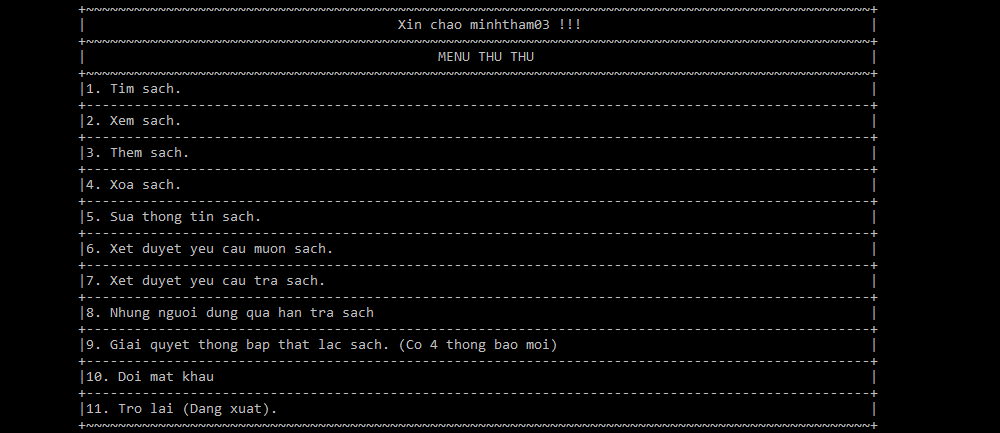
\includegraphics[width=18cm]{Images/menu_thuthu.png}
		\caption{MENU THỦ THƯ}
	\end{center}
\end{figure}

\begin{itemize}
	\item \underline{\textit{Thêm Sách}}\\
	Bạn có thể thêm sách với các thông tin sau: tên sách, thể loại, tác giả. Hệ thống sẽ tự đông cung cấp id sách bằng cách cộng id sách lần cuối cùng thêm vào với 1.
	\item \underline{\textit{Xóa sách.}}\\
	Bạn sẽ nhập id sách muốn xóa vào. Hệ thống sẽ xóa sách đó và sẽ reset lại tất cả các id sách lại theo thứ tự tăng dần. Ví dụ: Các id sách lần lượt là 1,2,3,4. Lúc này, bạn muốn xóa sách có id là 2 thì hệ thống sẽ xóa sách có id là 2 và reset lại cái id sách là 1,2,3.
	\item \underline{\textit{Sửa thông tin sách}}\\
	Hệ thống sẽ yêu cầu bạn nhập ID sách để có thể sửa thông tin của sách gồm tên sách, thể loại, tác giả.
	\item \underline{\textit{Xét duyệt yêu cầu mượn sách.}}\\
	Hệ thống sẽ in ra các yêu câu mượn sách của các độc giả. Các thông tin này bao gồm:
\begin{itemize}
	\item Tài khoản mượn sách.
	\item Danh sách mượn: ID sach, tên sách, số lượng mượn sách.
	\item Ngày mượn sách.
	\item Hạn cuối trả sách.
\end{itemize}
Ở đây bạn có thể chấp nhận từng yêu cầu, chập nhận tất cả yêu cầu và từ chối tất cả các yêu cầu đó.
	\item \underline{\textit{Xét duyệt yêu cầu trả sách.}}\\
	Hệ thống sẽ yêu cầu bạn nhập tên tài khoản trả sách và sẽ in ra ngày hiện tại của bạn trả sách là ngày nào. Nếu bạn muốn trả sách thì xác nhận yêu cầu này
	\item \underline{\textit{Những người dùng quá hạn trả sách.}}\\
	Hệ thống sẽ in ra danh sách các tài khoản đã quá hạn mượn sách. Bạn có thể nhập tên tài khoản mượn sách để gửi yêu cầu xử lý về việc quá hạn trả sách này.
	\item \underline{\textit{Giải quyết các thông báo thất lạc sách.}}\\
		Hệ thống sẽ tự động cho bạn biết có bao nhiêu yêu cầu xử lý việc thất lạc sách của độc giả gửi đến. \\
		Khi bạn chọn tính năng này hệ thống sẽ in ra các nguyên nhân của việc thất lạc sách của độc giả. Bạn có thể dựa vào đó mà gửi yêu cầu xử lý việc này.
\end{itemize}
\subsection{Menu dành cho Độc giả và quản lý người dùng}
\begin{figure}[htp]
	\begin{center}
		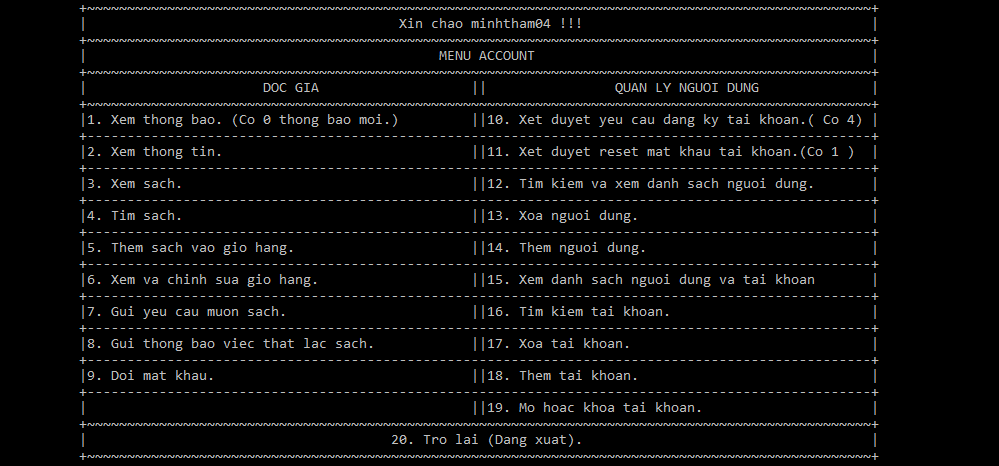
\includegraphics[width=18cm]{Images/menu_docgiavaquanlynguoidung.png}
		\caption{MENU ĐỘC GIẢ VÀ QUẢN LÝ NGƯỜI DÙNG}
	\end{center}
\end{figure}

\subsection{Menu dành cho Độc giả và thủ thư}
\begin{figure}[htp]
	\begin{center}
		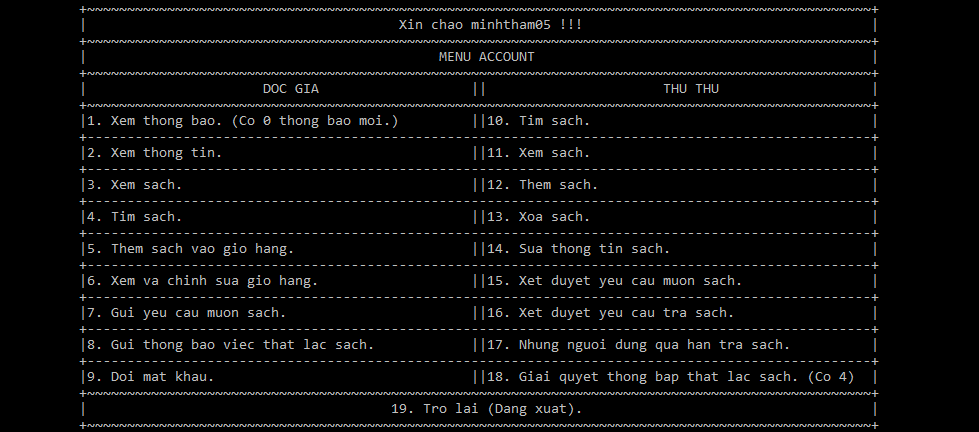
\includegraphics[width=18cm]{Images/menu_docgiavathuthu.png}
		\caption{MENU ĐỘC GIẢ VÀ THỦ THƯ}
	\end{center}
\end{figure}

\subsection{Menu dành cho Quản lý người dùng và thủ thư}
\begin{figure}[htp]
	\begin{center}
		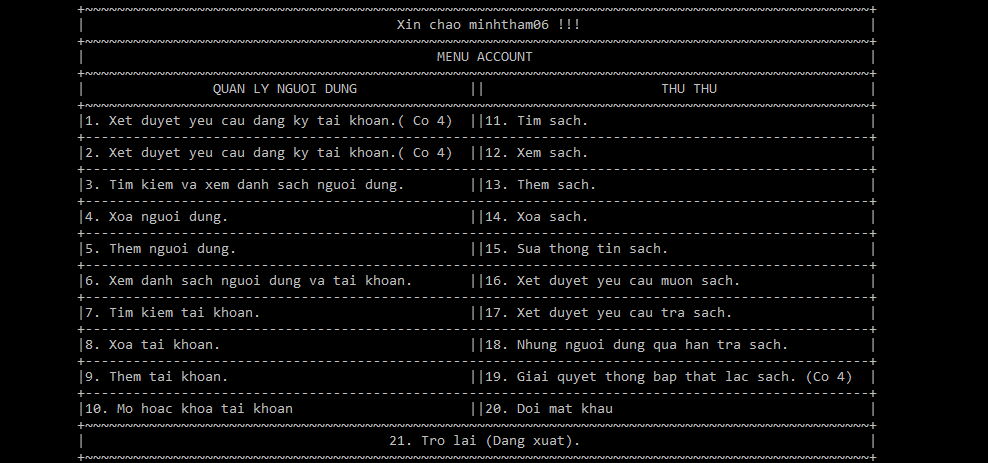
\includegraphics[width=18cm]{Images/menu_quanlynguoidungvathuthu.png}
		\caption{MENU QUẢN LÝ NGƯỜI DÙNG VÀ THỦ THƯ}
	\end{center}
\end{figure}
\subsection{Menu dành cho Độc giả, quản lý người dùng và thủ thư}
\begin{figure}[htp]
	\begin{center}
		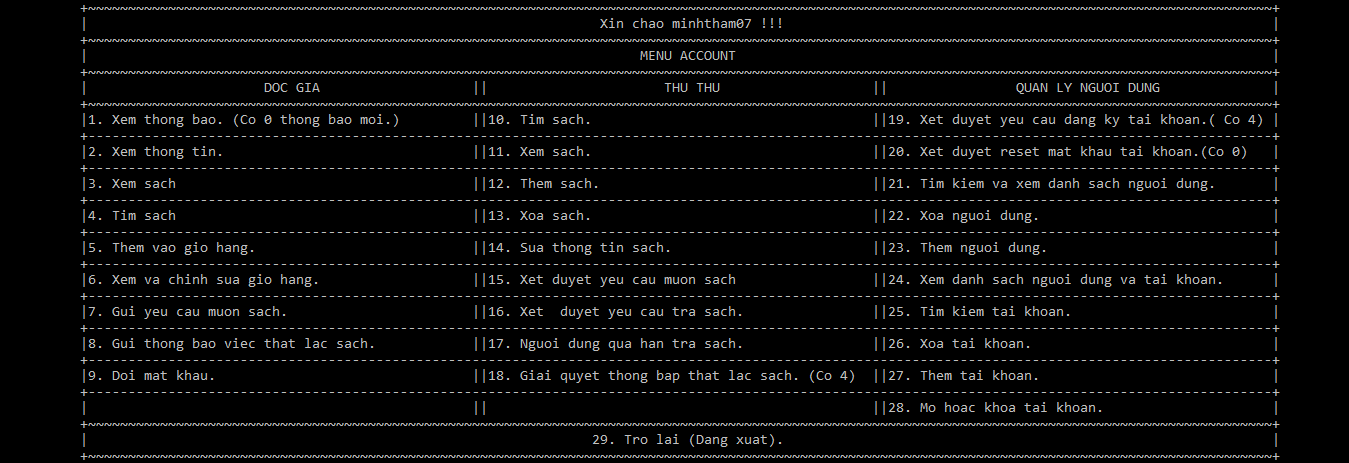
\includegraphics[width=18cm]{Images/menu_tatca.png}
		\caption{MENU CỦA TẤT CẢ VAI TRÒ}
	\end{center}
\end{figure}
\end{document}